\section{Experimental Protocol}
The experiments use a trial-averaged affective ERP dataset with 211 subjects after exclusion of one anomalous subject record. Each subject contributes three affective conditions: negative, neutral, and pleasant, yielding 633 subject-condition observations. The ERP traces contain 34 scalp channels sampled at high temporal resolution and baseline-corrected relative to stimulus onset. The primary task is three-class affective condition analysis. This task is not interpreted as a diagnostic decision problem; it is used as an external label structure for evaluating temporal representation under subject-level validation.

\section{Results}
\subsection{Clean Subject-Level Classification}
Table~\ref{tab:clean} reports clean three-class affective condition performance. The reservoir embedding does not dominate the classical baseline under clean static classification. This constrains the interpretation: the reservoir acts as a nonlinear temporal measurement operator, not as an automatically superior classifier.

\begin{table}[t]
\caption{Clean subject-level affective condition performance.}
\label{tab:clean}
\centering
\begin{tabular}{lccc}
\toprule
Configuration & Feature family & BA & Macro-F1 \\
\midrule
A0 & Classical bandpower/ERP & 0.485 & 0.483 \\
A1 & Reservoir embedding $E$ & 0.463 & 0.460 \\
A2 & Temporal descriptors $D$ & 0.432 & 0.428 \\
A6 & Reservoir + descriptors $E{+}D$ & 0.478 & 0.475 \\
\bottomrule
\end{tabular}
\end{table}

\subsection{Representation-Level Perturbation Response}
Table~\ref{tab:repr_perturb} summarizes representative feature-space perturbation results. Under additive amplitude corruption, the classical bandpower baseline degrades from BA $0.485$ to $0.395$ at 5 dB. The reservoir embedding degrades more weakly, from BA $0.463$ to $0.449$. A similar pattern occurs under feature dropout, where the reservoir embedding remains close to its clean value at 30\% dropout. Fig.~\ref{fig:perturbation} visualizes this contrast.

\begin{table}[t]
\caption{Representation-level perturbation diagnostics.}
\label{tab:repr_perturb}
\centering
\begin{tabular}{llccc}
\toprule
Perturbation & Level & A0 BA & A1 BA & Difference \\
\midrule
Clean & -- & 0.485 & 0.463 & -0.022 \\
Amplitude noise & 5 dB & 0.395 & 0.449 & +0.054 \\
Channel dropout & 30\% & 0.408 & 0.456 & +0.048 \\
\bottomrule
\end{tabular}
\end{table}

\begin{figure}[t]
\centering
% Figure source: representation-level perturbation response for BIBM 2026.
% Values are balanced accuracy from the manuscript tables.
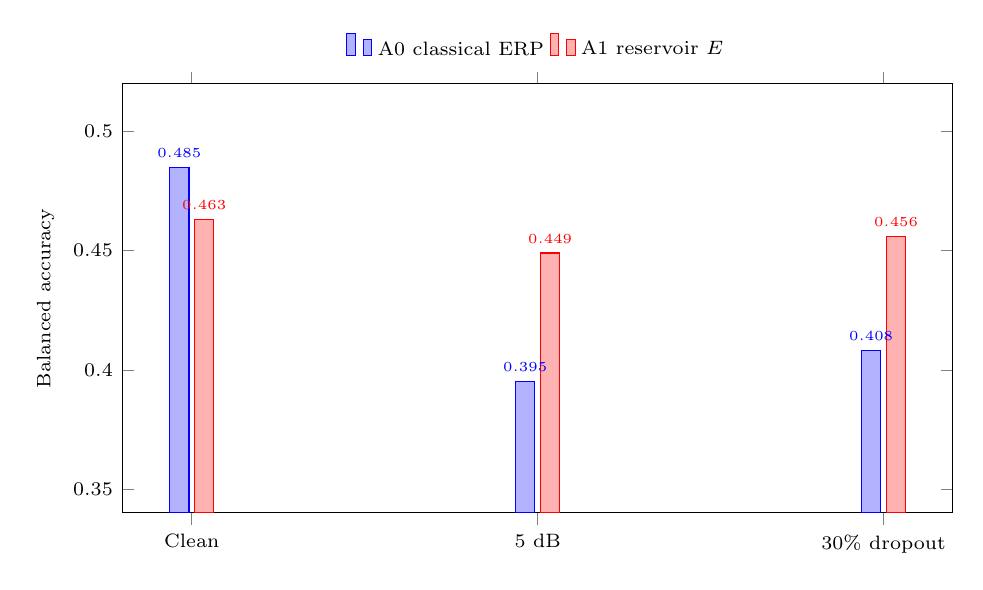
\begin{tikzpicture}
\begin{axis}[
    width=\linewidth,
    height=0.58\linewidth,
    ybar,
    bar width=7pt,
    ymin=0.34,
    ymax=0.52,
    ylabel={Balanced accuracy},
    symbolic x coords={Clean,5 dB,30\% dropout},
    xtick=data,
    x tick label style={font=\scriptsize, align=center},
    y tick label style={font=\scriptsize},
    label style={font=\scriptsize},
    legend style={font=\scriptsize, at={(0.5,1.03)}, anchor=south, legend columns=2, draw=none},
    nodes near coords,
    nodes near coords style={font=\tiny, /pgf/number format/fixed, /pgf/number format/precision=3},
    every axis plot/.append style={draw=black}
]
\addplot coordinates {(Clean,0.485) (5 dB,0.395) (30\% dropout,0.408)};
\addplot coordinates {(Clean,0.463) (5 dB,0.449) (30\% dropout,0.456)};
\legend{A0 classical ERP, A1 reservoir $E$}
\end{axis}
\end{tikzpicture}

\caption{Representation-level perturbation response for the classical ERP baseline (A0) and reservoir embedding (A1). The reservoir embedding has lower clean BA but retains BA more strongly under severe feature-space noise and dropout in this diagnostic regime.}
\label{fig:perturbation}
\end{figure}

\subsection{Raw-Signal Recomputed Perturbations}
A stricter test corrupts the signal before feature extraction and recomputes the representation. Table~\ref{tab:raw_perturb} reports a representative recomputation diagnostic. In this setting, temporal jitter and channel dropout produce larger degradation than the representation-level diagnostic because the perturbations alter the reservoir input trajectory before spike counts are formed.

\begin{table}[t]
\caption{Raw-signal recomputation perturbation diagnostic.}
\label{tab:raw_perturb}
\centering
\begin{tabular}{lcc}
\toprule
Condition & BA & Macro-F1 \\
\midrule
Clean recomputation subset & 0.433 & 0.415 \\
Temporal jitter, $\pm 50$ ms & 0.389 & 0.343 \\
Amplitude noise, 5 dB & 0.429 & 0.408 \\
Channel dropout, 30\% & 0.362 & 0.312 \\
\bottomrule
\end{tabular}
\end{table}
